\begin{figure}[!ht]
\begin{subfigure}{\linewidth}
\centering
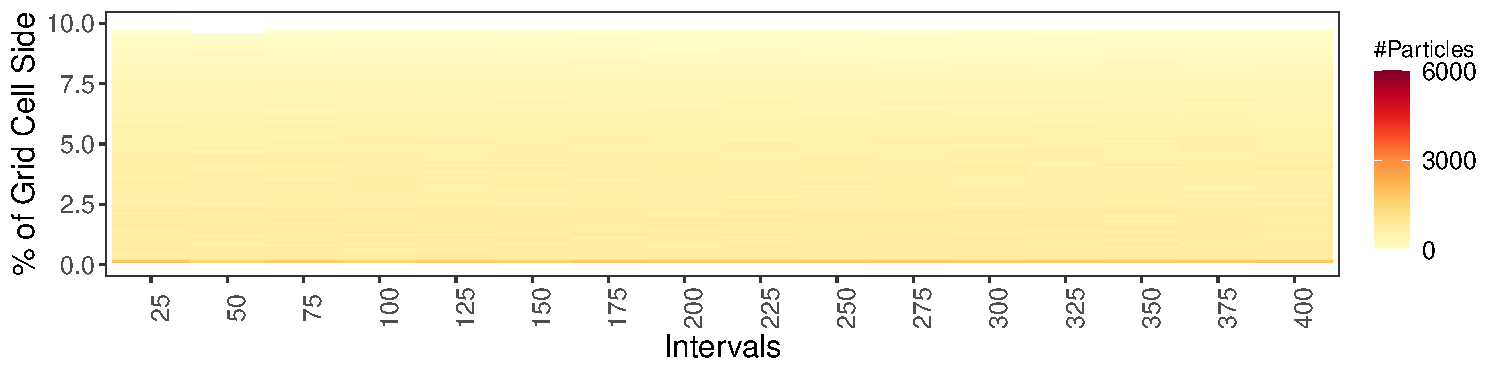
\includegraphics[width=\linewidth]{Images/ABC_Intervals_T4.pdf}
\vspace{-5mm}
\caption{T4, storage interval = 25 cycles}
\label{fig:abc_4}
\end{subfigure}
%\begin{subfigure}{\linewidth}
%\centering
%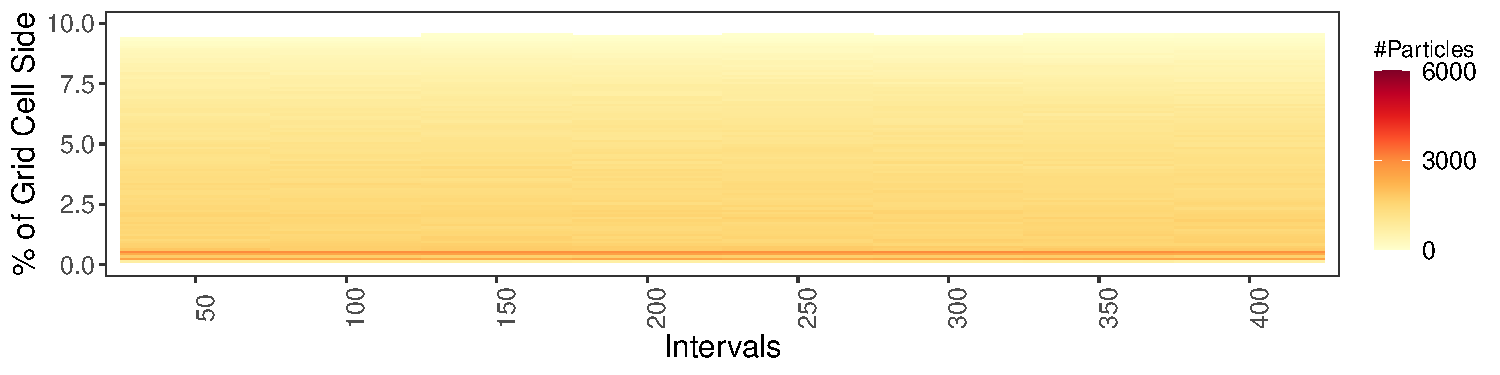
\includegraphics[width=\linewidth]{Images/ABC_Intervals_T5.pdf}
%\caption{T5, storage interval = 50 cycles}
%\label{fig:abc_5}
%\end{subfigure}
\begin{subfigure}{\linewidth}
\centering
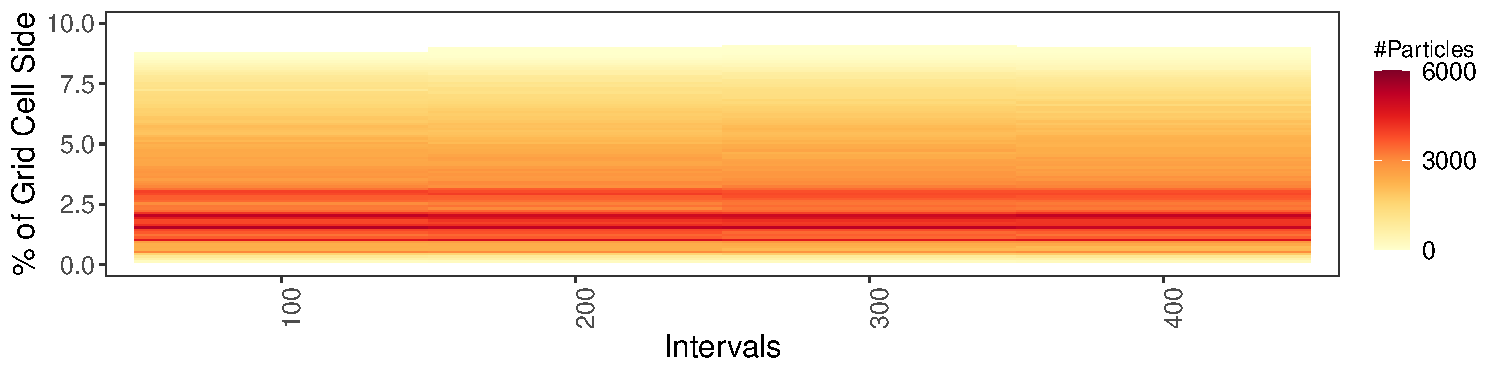
\includegraphics[width=\linewidth]{Images/ABC_Intervals_T6.pdf}
\vspace{-5mm}
\caption{T6, storage interval = 100 cycles}
\label{fig:abc_6}
\end{subfigure}
\caption{\fix{Reconstruction error for the ABC data set as a function of interval. This plot shows that the majority of reconstructed trajectories are within a grid cell side of the ground truth, despite the larger of number of discarded particles resulting from larger storage intervals.}}
%\caption{\fix{For the ABC data set, although increasing the storage interval resulted in a larger number of discarded particles, the majority of reconstructed trajectories are within a grid cell side of the ground truth.}} 
%\caption{ABC data set tests showing impact of variation in storage interval on the distribution of reconstruction error.}
\vspace{-5mm}
\label{fig:abc_map}
\end{figure}
